\chapter{Testing emergence for a small community}
\label{ch:extension}

In the previous chapter we addressed some \textit{ad hoc} design decisions made by \citet{deBoer2000}.
In this chapter, we present another extension on the original model by \citet{deBoer2000}.
Instead of using random selection for initiator and imitator pairs, we use a small-community-like network.
This network is based on 5 main groups of agents, each with different influences on the other.
The network can behave both vertical and horizontal, i.e. generational or not.
This extension is a demonstration of how the provided code can be used to easily configure new experiments.
This implementation is discussed step-by-step in the \texttt{4\_adding\_small\_communities} notebook.

%------------------------------------

\section{Small-community-like network}
\label{sec:network_idea}

\begin{figure}[H]
    \centering
    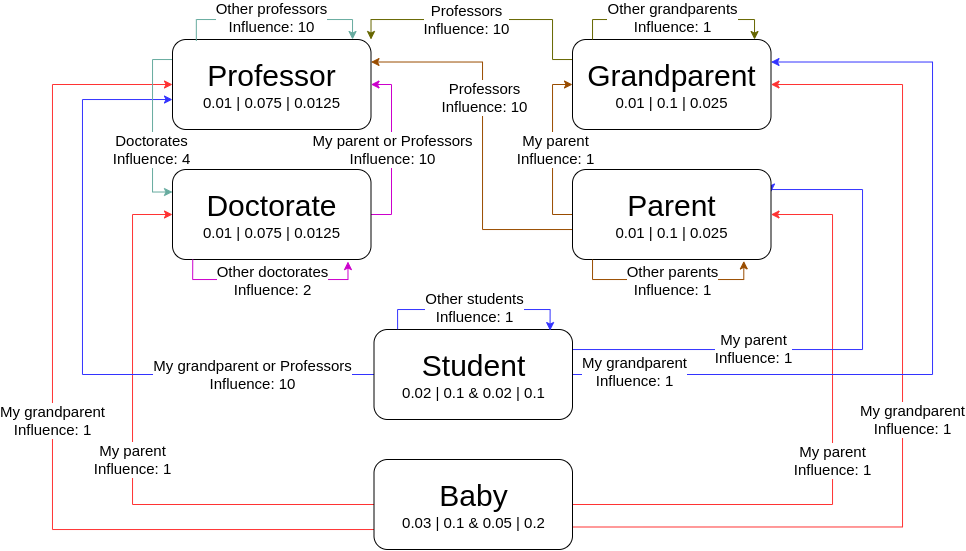
\includegraphics[width=\linewidth]{images/extension/network.png}
    \captionsetup{width=\linewidth}
    \captionsetup{justification=centering}
    \caption{Properties of small community network used.\\Arrows indicate an influential role for the agent accompanied by its weight.\\Notation underneath role: new sound probability $|$ ambient noise $|$ phoneme step size.}
    \label{fig:network}
\end{figure}

\newpage


%------------------------------------

\section{Community roles}
\label{sec:community_roles}

In Figure \ref{fig:network}, a general overview of the used network is shown.
From this diagram, it is visible that there are six different agent roles.
These roles are stored as an \texttt{Enum} under the \texttt{Community Role} class.
An agent will be one of these roles for a specified number of iterations.
This number is provided as the \texttt{category\_age\_width} parameter for the \texttt{Community Game Engine} discussed further down this report.
It is important to clarify that \texttt{Babies} and \texttt{students} don't exist together, rather in the first half of the provided age width parameter these agents are babies, and in the second half they evolve to become students.
Each agent has at most one unique parent, depending on if that agent is still alive or not.
The parent agent might also still have a parent, resulting in a grandparent for the youngest agent.
After the number of iterations is passed specified by the age width parameters, agents \textit{shift up} in this network and their role evolves.
That means that students become either doctorates or regular parents, determined by their own parent's role.
Doctorates become professors and parents become grandparents.
Professors and grandparents get replaced by new agents who start with an empty vowel repertoire.
These agents are all children of one unique parent agent or doctorate agent.
This keeps the distribution constant throughout the games.

It is noted that the role names were chosen to be intuitively comprehensible.
In the case of primitive humans, a similar structure was likely to exist, with professors being leaders of tribes for example.


%------------------------------------

\section{Community behaviour}
\label{sec:community_behaviour}

Besides a \texttt{Community Role}, an agent also has a \texttt{Community Behaviour}.
This behaviour describes multiple things:
\begin{itemize}
    \item The probability of adding a new sound. This is shown as the first number under the role name in the diagram.
    \item The synthesizer to be used. This allows specification of the ambient noise and optional agent noise to be used as described in section \ref{sec:reimplementing_producing}. The noise levels are given as the second number under the role name in the diagram. If two values are given, the second describes the agent noise.
    \item The phoneme step size as described in section \ref{sec:reimplementing_agents}. This is shown as the third number under the role name in the diagram.
    \item The roles that an agent is influenced by. This will be respected when choosing an initiator when this agent is an imitator. This is shown as arrows in the diagram.
    \item The strength of the above-described influence. This integer number represents the number of optimisation steps taken after playing a game with an agent of that role. It is given as the label of the arrows on the diagram.
    
\end{itemize}


%------------------------------------

\section{Updating the imitation game to work with the small community network}
\label{sec:updating_immitation_game}

Updating the classes discussed in Chapter \ref{ch:reimplementing} to work with the above described small community network and behaviour is relatively straightforward.
Due to the use of Python classes, it is possible to create a child class where functions can be re-implemented only if needed for the wished extension.
A nice example of this is the \texttt{Community Agent} class.
It inherits from the regular Agent class described in \ref{sec:reimplementing_agents} and takes the community role and behaviour as extra initialisation parameters.
By overwriting the \texttt{improve\_sound} function, a simple loop calling the original \texttt{improve\_sound} function can be made.
This loop iterates for a specified amount depending on the opponent's role influence strength.
This mechanism is thus the one to make the influence by agents of a certain role bigger than the others.
The opponent's role can be stored by creating an additional \texttt{prepare\_current\_game} function which is called before the game is played.
Likewise, a \texttt{change\_agent\_role\_and\_behaviour} function can be added to evolve the agent to its new form.
These simple changes are everything that is needed to adopt the agent class to work in the described network.

To call these additional functions and to evolve the agents on the correct iteration, the \texttt{Game Engine} was also updated to a \texttt{Community Game Engine} similarly.
On important thing to mention is that the \texttt{Community Game Engine} now ensures each agent plays exactly once as imitator every round.
The order in which this is done is randomised each time.
This had to be done to ensure equal ageing of agents.
A \texttt{Community Game State} and \texttt{Community Statistics} class was also created to provide additional plotting functionalities.
This consist of being able to plot and evaluate only the highly educated (professor and doctorate) or the regular educated (parent and grandparent) agents.
Figure \ref{fig:custom_plotting} shows an example of these plotting functionalities.

\begin{figure*}[ht]
    \centering
    \begin{subfigure}{.30\textwidth}
        \centering
        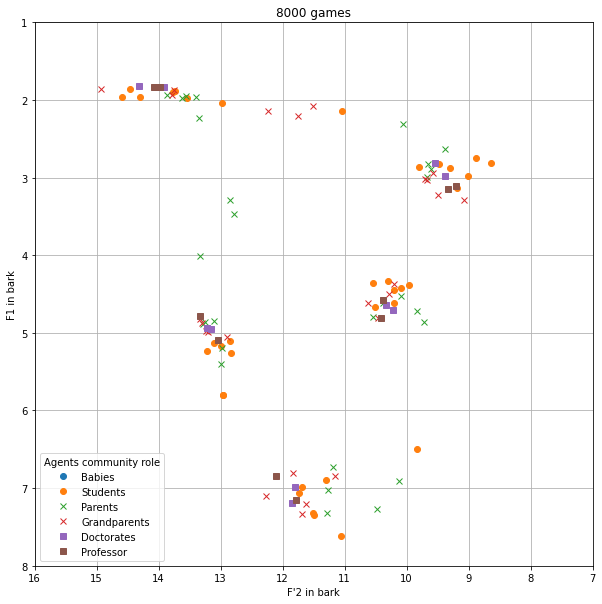
\includegraphics[width=\textwidth]{images/extension/sample_all.png}
        \captionsetup{width=0.9\linewidth}
        \captionsetup{justification=centering}
        \caption{All agents}
    \end{subfigure}
    \hspace{0.5cm}
    \begin{subfigure}{.30\textwidth}
        \centering
        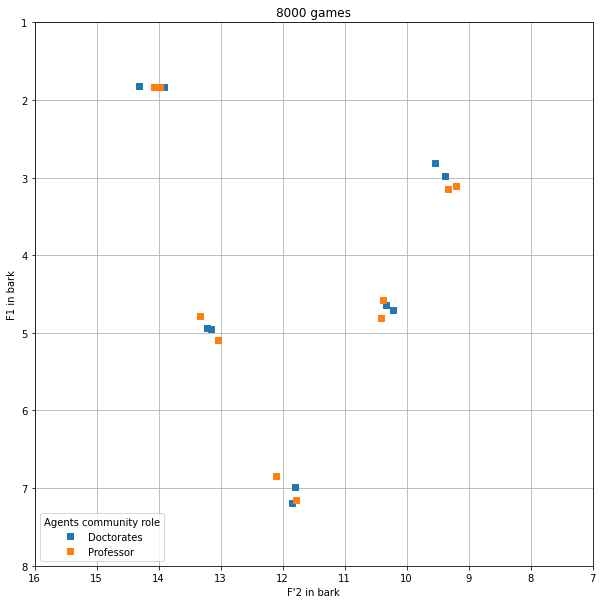
\includegraphics[width=\textwidth]{images/extension/sample_high.png}
        \captionsetup{width=0.9\linewidth}
        \captionsetup{justification=centering}
        \caption{Highly educated agents}
    \end{subfigure}
    \hspace{0.5cm}
    \begin{subfigure}{.30\textwidth}
        \centering
        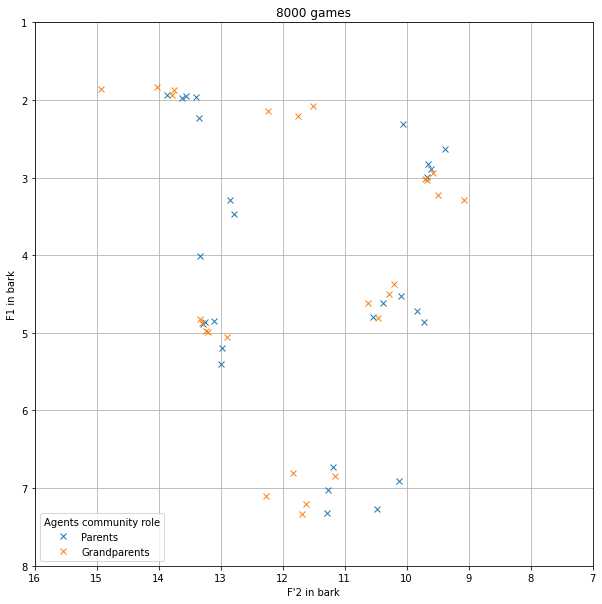
\includegraphics[width=\textwidth]{images/extension/sample_regular.png}
        \captionsetup{width=0.9\linewidth}
        \captionsetup{justification=centering}
        \caption{Regular educated agents}
    \end{subfigure}
    \captionsetup{width=0.9\linewidth}
    \captionsetup{justification=centering}
    \caption{Different plotting functionalities using the same game state object.}
    \label{fig:custom_plotting}
\end{figure*}